\documentclass[unnumsec,webpdf,modern,large]{mam-authoring-template}%

\usepackage[utf8]{inputenc}
\usepackage{amssymb,amsmath,latexsym}
\usepackage{soul,color}
\usepackage{xcolor}
\usepackage{graphicx,amssymb}
\usepackage{algorithm}
% \usepackage[noend]{algpseudocode}
% \usepackage{pgfplots}
% \usepackage{array}
\usepackage{anyfontsize}
\newcolumntype{P}[1]{>{\centering\arraybackslash}p{#1}}
\usepackage{tikz}
\usepackage{caption}
\setcounter{secnumdepth}{4}
\usepackage{hyperref}
\usepackage{float}
\usepackage{subcaption}
% \pgfplotsset{compat=newest}
%\usepackage{authblk}
% \usepackage{multirow}
\usepackage{url}
\usepackage[outdir=./]{epstopdf}   
\usepackage{dblfloatfix}
\usepackage[figuresright]{rotating}


% \graphicspath{{Fig/}}

% line numbers
%\usepackage[mathlines, switch]{lineno}
%\usepackage[right]{lineno}

% \theoremstyle{thmstyleone}%
% \newtheorem{theorem}{Theorem}%  meant for continuous numbers
% %%\newtheorem{theorem}{Theorem}[section]% meant for sectionwise numbers
% %% optional argument [theorem] produces theorem numbering sequence instead of independent numbers for Proposition
% \newtheorem{proposition}[theorem]{Proposition}%
% %%\newtheorem{proposition}{Proposition}% to get separate numbers for theorem and proposition etc.
% \theoremstyle{thmstyletwo}%
% \newtheorem{example}{Example}%
% \newtheorem{remark}{Remark}%
% \theoremstyle{thmstylethree}%
% \newtheorem{definition}{Definition}

\begin{document}

\firstpage{1}

\subtitle{Final Project for B.Sc. Degree in Computer Science}

\title[Accurate Landing of Drones]{Vision-Based Automatic Accurate Landing of Drones}

\author[1,$\ast$]{Shirel Zecharia}
\author[2]{Moria Grohar}

% \authormark{Author Name et al.}

\address[1]{\orgdiv{School of Computer Science}, \orgname{Ariel University}, \orgaddress{\street{Golan Heights 1}, \postcode{4077625}, \state{Ariel}, \country{Israel}}}


\corresp[$\ast$]{Project Mentors: Boaz Ben-Moshe, School of Computer Science, Ariel University; Or Haim Anidjar, School of Computer Science, Ariel University}


\abstract{This article introduces a platform designed to enable precise landings on the edge of rooftops, facilitating operations at boundary locations. The platform integrates voice recognition capabilities for activation, eliminating reliance on manual button controls. The primary objective is to develop a methodology and control algorithm that allows drones to guard settlements effectively. This research employs a combination of straight-line detection and object detection, avoiding the use of global positioning systems. The system is engineered to operate with drones equipped with existing cameras, obviating the need for additional sensors, and is implemented using the DJI SDK on Android devices. This paper presents a visual landing technology through a proposed algorithm, which is divided into two key tasks: scene evaluation and landing site security. Initially, the drone utilizes object detection to identify and avoid obstacles within the landing area, enabling autonomous descent planning. Once obstacles are cleared, the drone transitions to descent mode. For precise landings at the edge of a rooftop, an edge detection algorithm is employed alongside a target line selection process, allowing the user to designate a specific landing line beforehand, ensuring accuracy during the final approach.}

\keywords{Visual-Based Landing, Autonomous Landing, Accurate Landing, Spoken Language Recognition.}

\maketitle

\section{Introduction}
Unmanned aerial vehicles (UAVs), commonly known as drones, are aircraft that operate without an onboard pilot, controlled either through radio remote systems or autonomous onboard programs. Drones are valued for their simple yet effective design, ease of operation, flexibility, and cost-efficiency, making them versatile tools in both military and civilian domains. In military operations, drones play pivotal roles in tasks such as tactical reconnaissance, territorial surveillance, and target acquisition. In surveillance missions, accurate landing is especially critical, as drones must often be deployed to specific vantage points—such as rooftops or elevated positions—where stable operation is essential for continuous monitoring of target areas.\\
On the civilian side, drones are utilized for activities like environmental monitoring, weather data collection, and infrastructure inspection. As drones become increasingly prevalent in both sectors, ensuring their safe and precise landing—particularly in challenging environments—has emerged as a critical concern. In surveillance operations, an accurate landing ensures that drones can be positioned optimally to capture and monitor sensitive areas over extended periods, thus reducing the need for human intervention and minimizing the risks associated with miscalculation during deployment.\\
Autonomous drone operations have rapidly advanced, yet precision landing remains a significant challenge, especially in environments where GPS signals are unreliable or unavailable. GPS signals can be easily disrupted by various factors: (a) weather conditions and sunspots may weaken signals, although they typically do not hinder positioning; (b) electromagnetic interference from sources like radios and strong magnetic fields can cause varying degrees of disruption; (c) signal strength diminishes under shelters such as buildings, vehicles, insulation materials, trees, and metal components; and (d) high-rise buildings and dense urban areas can severely impact GPS signal quality. Traditional drone landing methods often rely on GPS, which proves inadequate in urban or indoor settings. This limitation poses significant challenges for applications requiring precise landings, such as military surveillance, urban package delivery, infrastructure inspection, and emergency response. As a result, there is a critical need to develop autonomous positioning and flight control systems for drones that do not rely on GPS signals.\\
This research addresses these challenges by developing a visual-based landing system that enhances accuracy and safety. Our approach enables drones to autonomously identify and land on strategic surfaces, such as rooftops, relying solely on visual data from the onboard camera. By eliminating the need for additional sensors or external data inputs, this system offers a robust solution for autonomous landings in complex environments, ensuring the drone is precisely positioned for effective surveillance and monitoring.

\section{Authors Contribution}\label{sec2}
We propose a visual processing framework that enables the drone to land autonomously by utilizing object (obstacle) detection and edge detection. Our approach is tested on a DJI drone equipped with a standard camera, using the DJI SDK for implementation on Android devices. Additionally, we have implemented a "guard" mode in the app — a button that, when activated, is designed to detect movement (such as people, cars, etc.) and send alerts. The system's robustness is further enhanced by incorporating basic voice commands through a speech recognition module, meeting the requirements outlined by MAFAT.

\section{Related Work}\label{sec3}
\subsection{Obstacle Avoidance}
Obstacle avoidance is a critical aspect of autonomous drone operations, especially in dynamic environments where both static and moving obstacles are present. One approach is integrating depth images with an occupancy voxel map to detect and track dynamic obstacles \cite{xu2023real}.
This approach effectively balances computational efficiency with the need for accurate detection and tracking, making it suitable for real-time UAV operations. Another approach involves deep learning techniques like the YOLO (You Only Look Once) framework, which excels at real-time obstacle detection in dynamic environments \cite{redmon2017yolo9000}. YOLO9000 enables rapid detection of multiple objects, making it ideal for fast decision-making in complex surroundings. Its efficiency and accuracy have made it a popular choice for enhancing UAV obstacle avoidance systems.

\subsection{Motion Detection and Object Detection: Yolo (You Only Look Once)}
Recent advancements in motion and object detection have been significantly influenced by the YOLO (You Only Look Once) framework. As highlighted by \cite{dahirou2021motion}, YOLO enables real-time object detection by predicting bounding boxes and class probabilities from full images in a single evaluation, enhancing both speed and accuracy. This capability makes YOLO particularly effective for applications requiring immediate responsiveness, such as surveillance and autonomous navigation.

\subsection{Speech Recognition}
Speech recognition has been explored as a key component in enhancing drone operation through voice commands, particularly in environments where manual control is impractical. Various systems have been developed for continuous speech recognition on Android devices, such as the one proposed by Srivastav et al. \cite{SpeechRecognition}, which enables real-time voice command processing for mobile platforms.
This technology is critical for integrating human-drone interaction, especially in hands-free scenarios, allowing operators to issue commands without physical intervention. Such advancements enable drones to act upon voice inputs for tasks like navigation, object detection, or activation of specific modes. Similar systems have been implemented to facilitate the control of unmanned aerial vehicles (UAVs) in real-time, optimizing human-machine interaction and expanding the use cases for drones in dynamic, complex environments.

\subsection{A Robust and Accurate Landing Methodology for Drones on Moving Targets}
Recent work has explored the use of ArUco markers for precision landing in autonomous drones, offering an efficient visual processing solution for target detection and tracking. As demonstrated in \cite{drones6040098}, ArUco markers provide high accuracy in identifying landing zones, especially when combined with robust visual algorithms. This approach addresses common challenges such as variable lighting conditions and drone stability during descent. Implementing these markers has shown success in enhancing landing precision, contributing to safer and more reliable autonomous operations.

\subsection{Vision-Based Autonomous Landing for the UAV}
In their review of vision-based autonomous UAV landings \cite{aerospace9110634} categorize landing scenarios into static, dynamic, and complex. Static landings often use cooperative targets like barcodes or fiducial markers for accurate positioning, while dynamic landings include vehicle- and ship-based platforms. The authors emphasize the challenges of real-time processing, limited onboard resources, and UAV maneuverability, noting that complex environments remain a significant research focus, with future work aimed at multi-sensor fusion and algorithmic adaptability.

\subsection{An improved Canny edge detection algorithm}
Edge detection algorithms play a critical role in enhancing the visual processing capabilities of drones by accurately identifying boundaries and objects within an image. The Canny Edge Detection Algorithm, as discussed in \cite{rong2014improved}, has proven to be highly effective due to its ability to detect edges with minimal noise while maintaining high accuracy. This method ensures that drones can detect and track obstacles, aiding in precise navigation and autonomous landing. Its application in real-time drone systems highlights its importance in improving the robustness of visual navigation and obstacle avoidance.

\section{Drone Control Mechanisms} \label{sec:mechanisms}
\subsection{Drone Control Parameters}
The drone’s movement is governed by four fundamental control parameters: yaw, pitch, roll, and throttle.
These parameters allow the drone to maneuver in 3D space with precision, facilitating both object tracking and navigation during various flight operations.

\textbf{Yaw} - controls the rotation around the vertical axis, allowing the drone to turn left or right to face objects.

\textbf{Pitch} - adjusts the forward and backward tilt, moving the drone in those directions.

\textbf{Roll} - manages side-to-side tilt, shifting the drone left or right.

\textbf{Throttle} - regulates altitude by increasing or decreasing the drone’s lift.

\subsection{Remote Controller Overview} \label{sec:RemoteControllerOverview}

The remote controller is crucial for operating a drone, allowing the pilot to manage flight characteristics effectively. Key features include:

(a) Joysticks - The left joystick controls throttle and yaw, while the right joystick manages pitch and roll, enabling intuitive movement and orientation.

(b) Buttons and Switches - Various buttons activate functions such as takeoff, landing, camera capture, and flight mode adjustments, enhancing operational versatility.

(c) Display Screen - Many controllers include a screen or connect to mobile devices to provide real-time telemetry, such as altitude, speed, and battery status, improving situational awareness.

(d) Communication Protocol - The controller communicates with the drone via RF signals, ensuring reliable connectivity and minimal latency during flight.


\subsection{Drone Sensors} \label{sec}

Drones utilize various sensors to enhance stability, navigation, and functionality during flight. Key sensors include:

\begin{description}

\item $\bullet$ Barometers - Measure atmospheric pressure to determine altitude. By monitoring changes in pressure, barometers help the drone maintain a steady altitude, which is essential for stable flight and landing.

\item $\bullet$ GPS (Global Positioning System) - Provides location data, enabling the drone to navigate to specific coordinates, maintain its position, and return to home automatically. GPS is vital for autonomous flight operations.

\item $\bullet$ Vision Sensors - Include cameras and optical flow sensors, allowing the drone to detect and track objects, recognize surfaces, and assist in navigation by analyzing visual data. These sensors are essential for tasks like object avoidance and following lines during autonomous flight.

\item $\bullet$ Ultrasonic Sensors - Measure distance to the ground using sound waves, aiding in altitude control and collision avoidance during low-altitude flights.

\end{description}

Together, these sensors provide the necessary data for the drone's flight controller to make real-time adjustments, ensuring stable and responsive flight even in challenging conditions.


This combination of controls and displays enhances the pilot's ability to maneuver the drone accurately and safely.


\section{Experimental Setup} \label{Experimental Setup}

\subsection{Hardware Used:}
For all flight operations, the DJI Mavic Air 2 was employed, utilizing its standard camera and onboard sensors. The drone's ability to control yaw, pitch, roll, throttle, and altitude played a crucial role in the testing and experiment execution.

\subsection{Testing Environment}

The experiments were conducted in both indoor and outdoor environments. For outdoor tests, the drone was operated in real-world conditions, including on the ground and atop a table, to simulate different elevation scenarios. Additionally, the DJI Mavic Air 2 was tested in varying weather conditions, including strong winds and sunny days, to assess its performance under challenging conditions.\\
To supplement the real-world tests, a simulator was employed to thoroughly evaluate the drone’s behavior and command responsiveness in a controlled, non-real-world-based environment. This simulation allowed us to test the system's reaction to flight commands, such as takeoff, landing, edge detection, and obstacle avoidance, in a reproducible setting without the risks associated with physical testing.\\
By testing in both simulated and real environments, the drone's flight stability and command accuracy were evaluated under diverse conditions, ensuring robustness and reliability in practical applications.
\subsection{Application View}
\begin{figure}[H]
    \centering
    \includegraphics[width=0.55\textwidth]{landingMainExplenation.png}  % Reduced the size here
    \caption{Landing view screen while running the app.}
    \label{fig:landingMainExplenation.}
\end{figure}
\section{Algorithm Design} \label{sec:algorithm}

Our proposed algorithm for autonomous drone landing consists of three key components: Target Line Selection, Flight Control, and Object Detection. Each part contributes to the overall reliability and precision of the landing process, ensuring safe navigation and obstacle avoidance.
Our algorithm utilizes the camera mounted on a gimbal angled at 45°.
\begin{figure}[H]
    \centering
    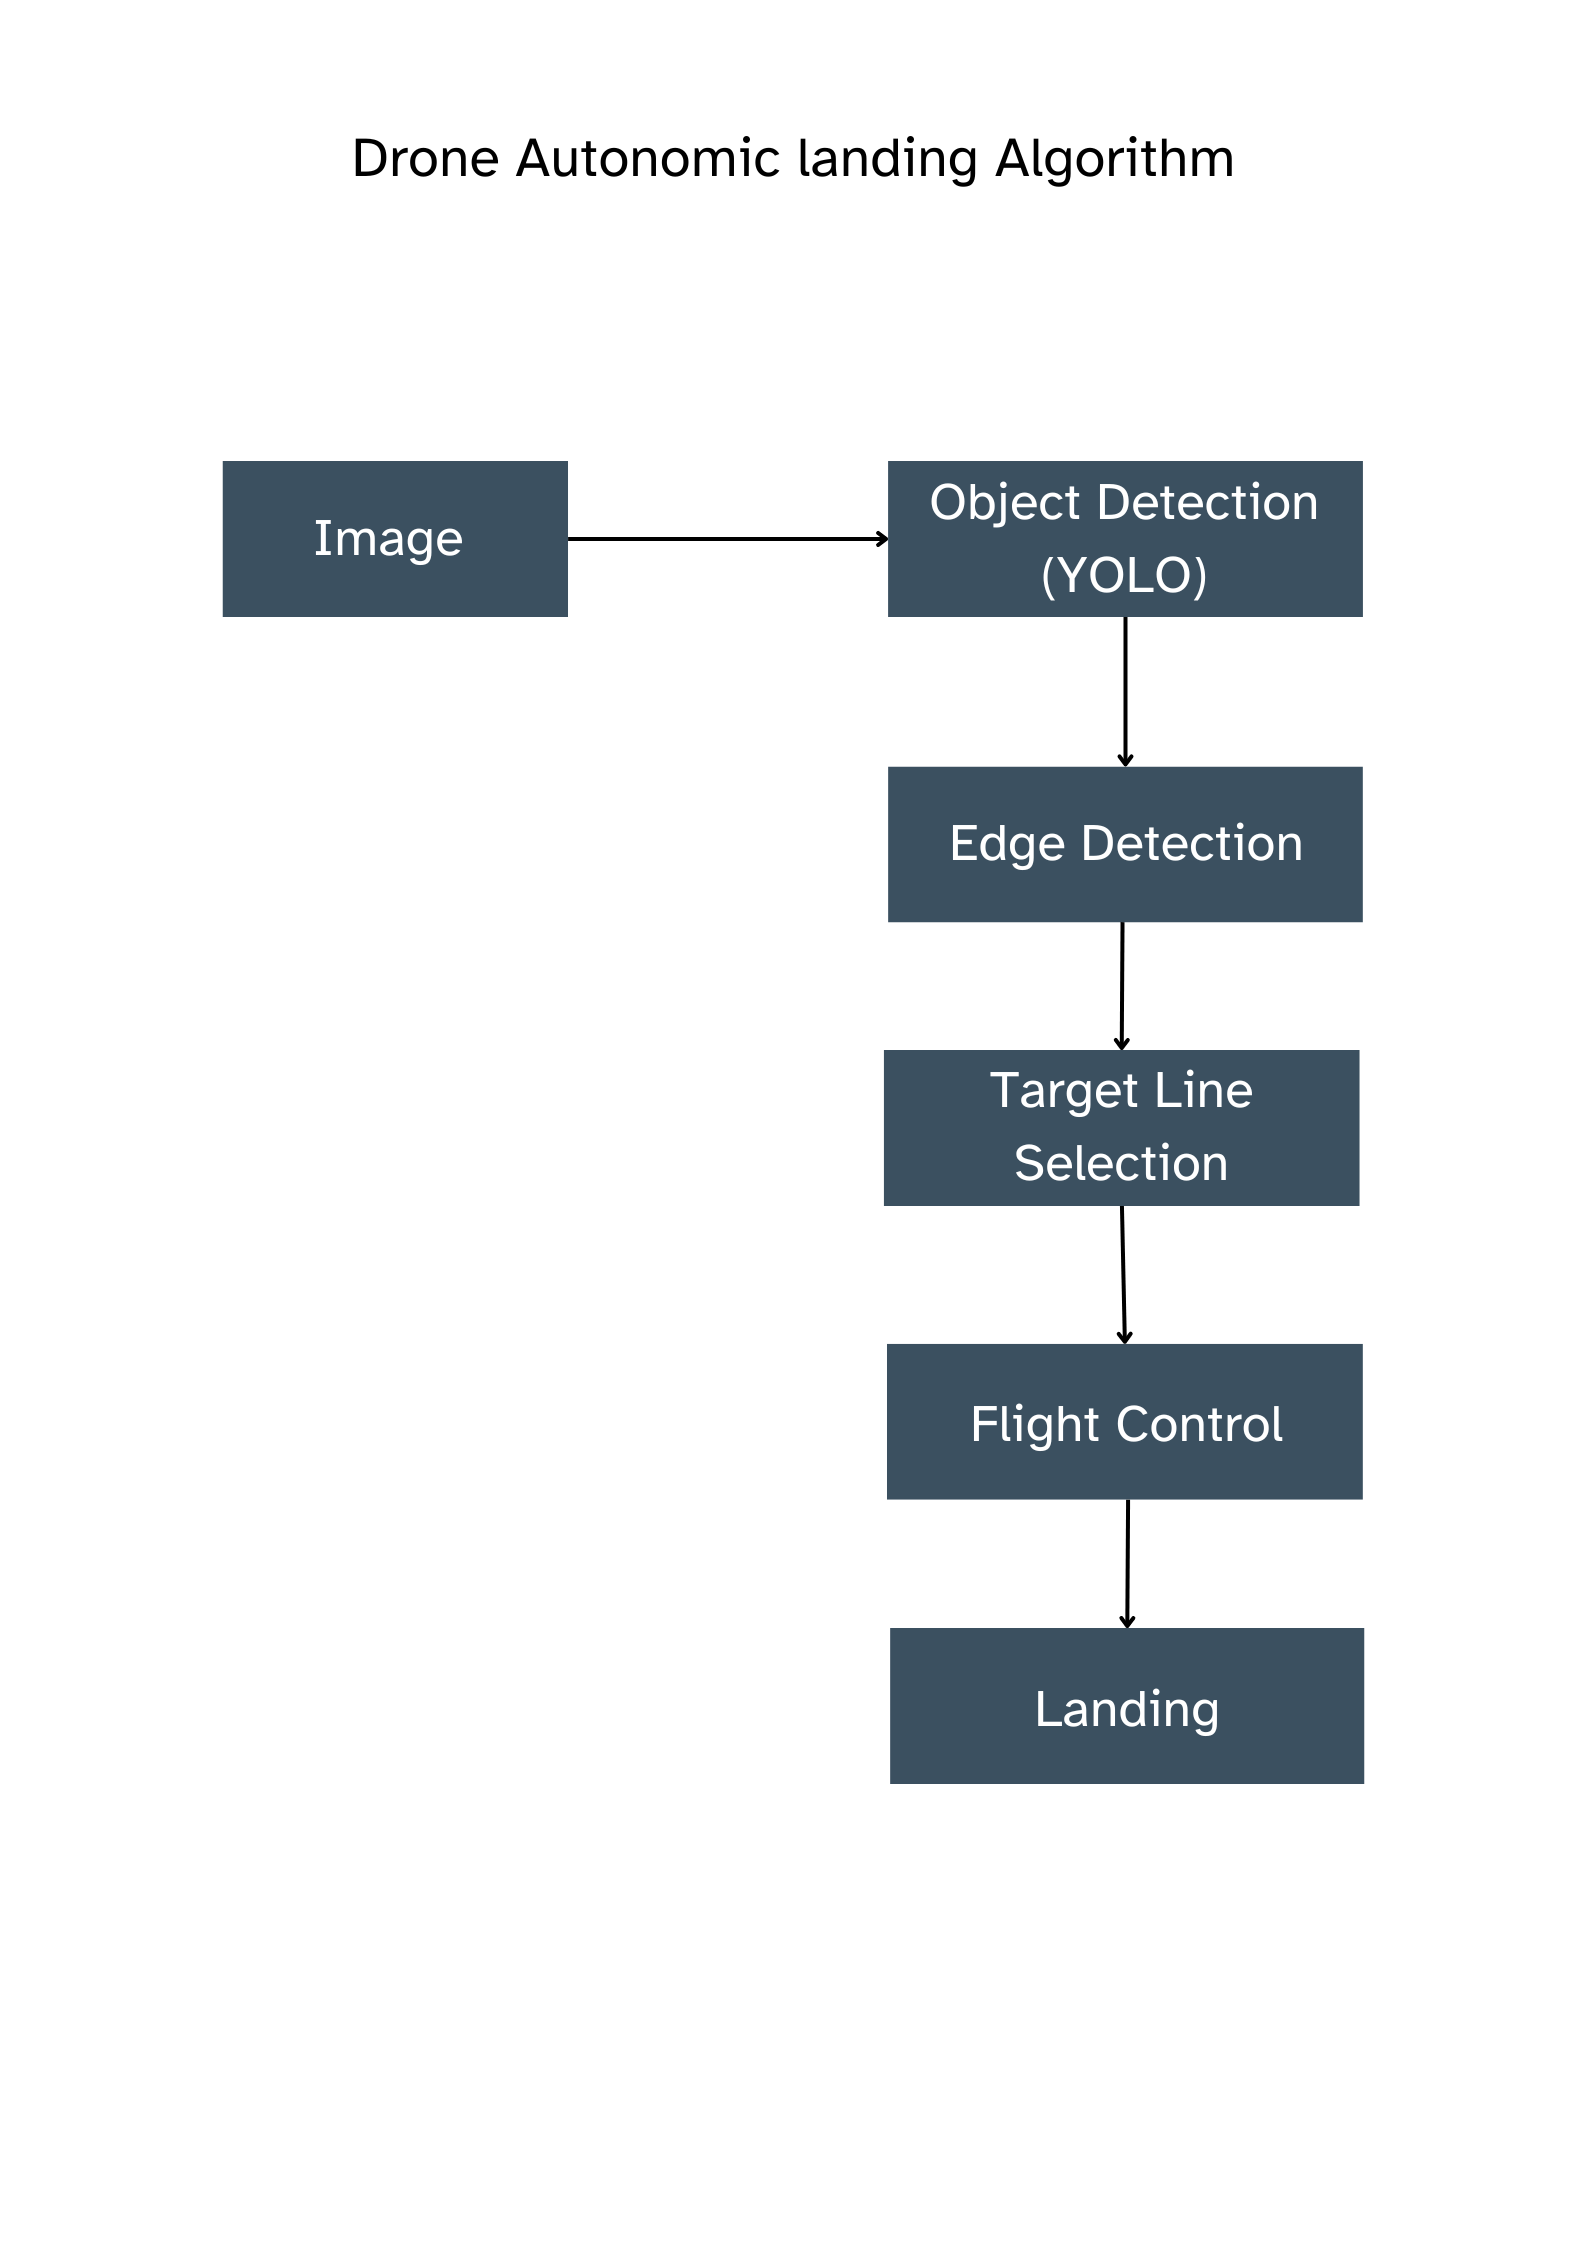
\includegraphics[width=0.48\textwidth]{Schematic_for_automatic_landing.png}  % Reduced the size here
    \caption{Schematic for automatic landing.}
    \label{fig:Schematic_for_automatic_landing.}
\end{figure}

\subsection{Target Line Selection}
In the first stage of the landing process, edge detection is activated to identify all available and compatible lines within the camera's field of view. These lines represent potential landing paths. The user interacts with the system by selecting the desired line for the drone to land behind via a touch-based interface. Once the target line is chosen, the algorithm continuously tracks the line. This is achieved by calculating the distance between the selected line and all detected lines, and the one with the minimum distance is updated as the current target line. This real-time tracking ensures that the drone can maintain accurate navigation towards the desired landing area.

\subsection{Flight Control}
After target line selection, the system activates the flight control module. The drone begins moving towards the selected line by issuing pitch commands, which direct forward movement. This continues until the chosen line is nearly out of the drone’s visible range. Through experimental measurements, we identified a blind spot between the drone's final visible position of the line and its actual location in reality.
To compensate for this, the algorithm uses the ratio $$ R=\frac{h}{d}$$, where $h$ is the drone’s height and $d$ is the blind spot distance, to calculate the necessary adjustment.
For diagonal movement at a 45° angle, the pitch (horizontal) and throttle (vertical) inputs must result in equal movement. The blind spot ratio R is used to balance them: $$R = \frac{throttle\_value}{pitch\_value}$$ Here, the throttle value is adjusted according to the drone's height, ensuring accurate diagonal movement and blind spot compensation. A final pitch command ensures the drone reaches the correct position relative to the target line.

\begin{figure}[H]
    \centering
    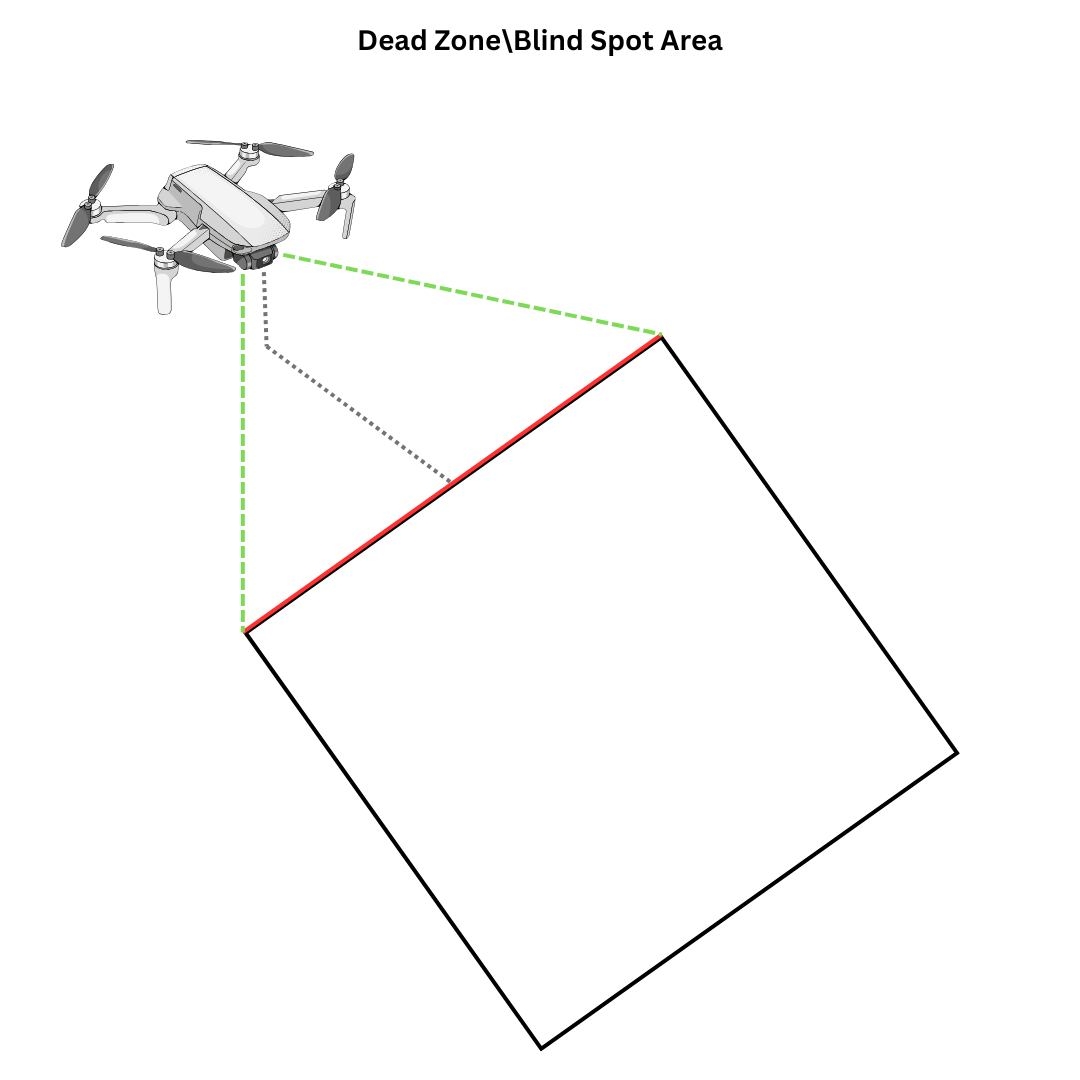
\includegraphics[width=0.5\textwidth]{Blind Spot Area.png}
    \caption{Blind Spot Area.}
    \label{fig:Blind Spot Area.}
\end{figure}

\subsection{Object Detection}
Upon reaching the target area, object detection is initiated to scan for potential hazards in the intended landing zone. The detection algorithm examines the area for obstacles such as people, vehicles, or other objects that may hinder safe landing. The landing zone's dimensions are calculated based on prior measurements from different drone positions, ensuring the detection area is appropriately scaled for accurate hazard identification. If no hazards are detected, the system proceeds with the landing sequence, ensuring a safe and precise touchdown.

\section{Movement Detection}
An important aspect of this project is the integration of movement detection, designed to enhance the drone’s functionality as a surveillance tool. Once the drone has landed on a designated edge, it operates as a stationary surveillance camera. In this mode, the system continuously monitors the surrounding environment for movement.\\
Movement detection is implemented using the YOLO (You Only Look Once) object detection framework, which enables real-time identification of objects such as people, vehicles, or other moving entities. When movement is detected, the system immediately alerts the user through the app. This alert includes both a voice notification, specifying what has been detected, and a text message displayed on the screen. These alerts provide real-time updates, enabling timely responses to any potential security concerns.

\begin{figure}[H]
    \centering
    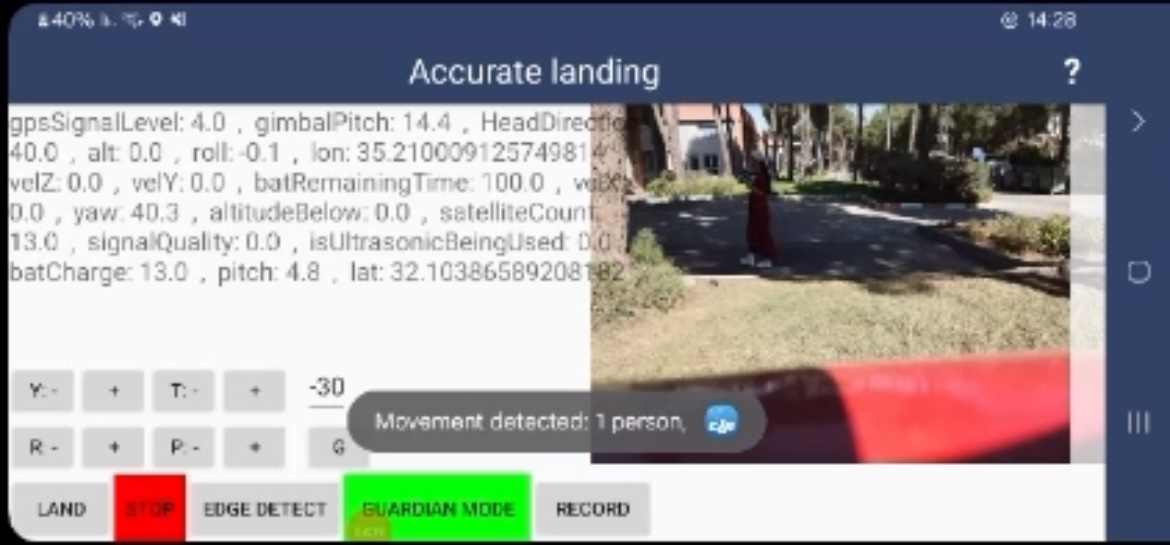
\includegraphics[width=0.5\textwidth]{movementDetect.png}  % Reduced the size here
    % \caption{Guardian mode activated.}
    \label{fig:movementDetect.}
\end{figure}

\section{Speech Recognition} \label{sec:SpeechRecognition}
The speech recognition system, powered by Google Speech Recognition, continuously listens for the user’s voice until it detects the wake word "hey rexi." Once activated, the system checks subsequent speech for commands from the predefined list, enabling real-time control of the drone without touching the screen. This approach allows the system to remain responsive while minimizing unnecessary processing, facilitating a hands-free operation experience.

Each recognized command triggers a specific action in the drone. The key commands and their associated actions are:

(a) \textbf{Takeoff} - Initiates the drone's takeoff sequence, lifting it to a designated altitude for hover.

(b) \textbf{Land} - Initiates the landing sequence, lowering the throttle for a controlled descent until the drone reaches the ground.

(c) \textbf{Stop} - Halts any current movement, keeping the drone stationary in hover mode.

(d) \textbf{Move up} - Increases the throttle to elevate the drone vertically.

(e) \textbf{Move down} - Decreases the throttle, causing the drone to descend.

(g) \textbf{Start recording} - Begins video recording using the drone's camera.

(h) \textbf{Stop recording} - Stops the video recording and saves the footage.

(i) \textbf{Edge detection} - Activates the edge detection algorithm, allowing the system to identify and process edges for navigation or object tracking.

(j) \textbf{Movement detection (Guard Mode)} - Activates a security or surveillance mode where the drone monitors for movement in its environment and triggers alerts or actions based on detected motion.

(k) \textbf{Start movement detection} - Begins monitoring the environment for movement.

(l) \textbf{Stop movement detection} - Disables the movement detection and returns to normal operation.

This combination of commands allows users to control the drone in various situations, from basic navigation to more advanced functionality, such as edge detection and movement detection for security or surveillance purposes.

\section{Future Work} \label{sec:future}
An important area for future improvement is the algorithm's ability to handle wind conditions, particularly in outdoor environments and at higher altitudes. While the current implementation performs reliably in controlled settings, real-world scenarios—such as fluctuating wind speeds and changing directions—pose significant challenges to the drone's stability and landing accuracy. Specifically, turbulence at great heights can disrupt the drone's trajectory, leading to deviations from the intended flight path and reducing the precision of both target line tracking and landing position.\\
To address these challenges, we plan to enhance the algorithm by integrating real-time wind compensation techniques. This improvement will involve adapting the flight control module to account for external forces, using sensor and visual data to counteract wind disturbances, and dynamically adjusting the drone's movements. Enhancing wind handling will enable the algorithm to perform more reliably across a wider range of scenarios, ensuring consistent operation in varying environmental conditions.\\
Additional future work includes transitioning the speech recognition system from an online to an offline model, which will improve reliability by ensuring consistent functionality without internet access. Furthermore, we plan to explore the integration of plane recognition algorithms to enhance landing precision. This capability will enable the drone to autonomously identify suitable landing surfaces, thus increasing safety and operational efficiency.

\section{Conclusion}
In this work, we presented a novel approach for autonomous drone landing using a visual-based framework that eliminates the need for GPS.\\
Our algorithm, tested on a DJI drone equipped with a standard camera, successfully integrates object detection, edge detection, and flight control to enable precise landings. \\
The system's performance in controlled environments demonstrates its effectiveness, especially in scenarios where GPS signals are unreliable or unavailable.\\
However, there are still challenges to address, particularly in handling unpredictable wind conditions and ensuring the system’s reliability in diverse outdoor environments.\\
Future work will focus on improving the algorithm’s robustness in real-world scenarios and enhancing its functionality through additional features such as offline speech recognition and plane recognition algorithms for safer and more autonomous landings.\\
The combination of these developments will pave the way for safer, more reliable, and efficient drone operations in a wide variety of applications, from urban package delivery to military surveillance missions.

\bibliographystyle{plain}
\bibliography{myDoc}       
\end{document}